\section{Implementation and Evaluation}
\label{sec:evaluation}

\begin{figure}[t]
    \centering
    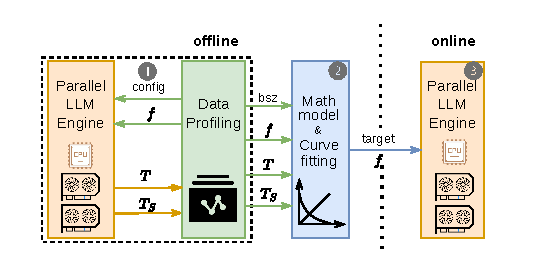
\includegraphics[width=0.8\linewidth]{figures/TACO_Rebuttal/overview_new.pdf}
    \caption{The deployment of \thisproj{}. In the Offline Phase, critical parameters are collected to construct an analytical model. In the Online Phase, the GPU frequency is adjusted based on the model's guidance. }
    \label{overview}
\end{figure}

% We have implemented \thisproj{} on the open-source SARATHI framework \cite{agrawal2024taming} and choose it as baseline.
% SARATHI is built on the widely used LLM inference framework vLLM \cite{kwon2023efficient}, which is the first open-source framework to adopt the continuous batching technique.
% Additionally, SARATHI provides APIs to record the lifecycle of each request in detail, enabling precise data collection and profiling.

\bylyz{
We have implemented \thisproj{} on the open-source SARATHI and SGLang framework.
The former is built on the vLLM and provides AIPs to record the lifecycle of each request in detail for data collectiong and profiling.
The latter is another widely used LLM inference framework, mainly used for XXX.
}

% \begin{figure}[t]
%     \centering
%     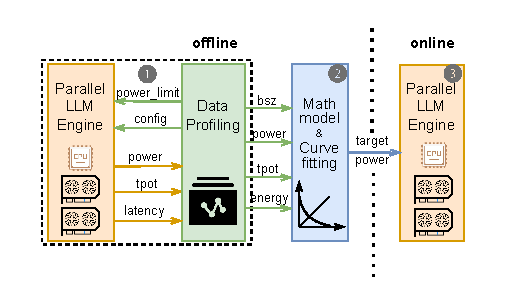
\includegraphics[width=0.7\linewidth]{figures/overview.pdf}
%     \caption{The deployment of \thisproj{}. In the Offline Phase, critical parameters are collected to construct an analytical model. In the Online Phase, the GPU power cap is adjusted based on the model's guidance. }
%     \label{overview}
% \end{figure}

Figure~\ref{overview} shows the implementation and the deployment of the \thisproj{}. 
It consists of two main components: the offline profiling part and the online frequency adjustment part.
During offline profiling part, the deployed LLM engine processes a small number of requests to collect the data for $T_S$ and $T$ under different frequency settings. 
Accordingly, the parameters for the \textit{TFPrediction Model} can also be derived from the collected data. 
Using the method outlined in Section~\ref{sec:guide}, the optimal frequency settings are then determined. 
The model and its setting can be reused for the same model configuration running on the hardware platforms with the same features later.
During online frequency adjustment part, the frequency is configured before the inference process begins, after which the system can operate without further intervention.

% \begin{figure*}[t]
%     \centering
%     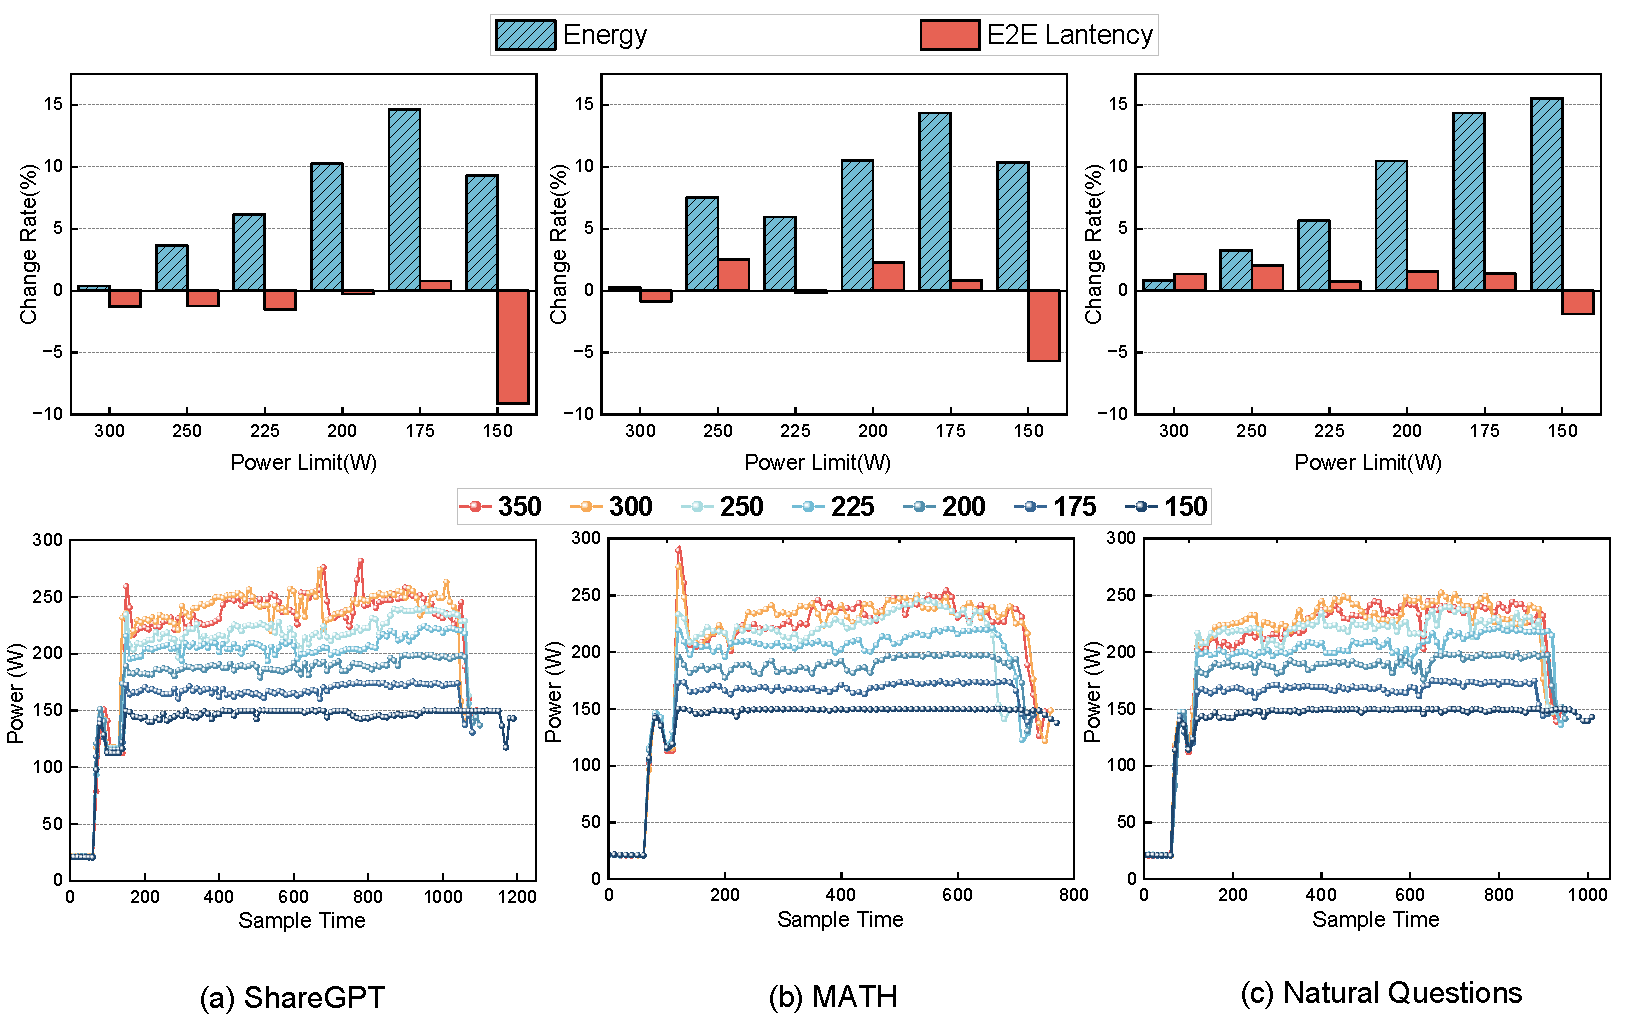
\includegraphics[width=\linewidth]{figures/power_lantency.pdf}
%     \caption{Energy savings and performance variations at different power levels across multiple datasets using the Llama2-7B model. Positive numbers indicate improved performance, while negative numbers indicate decreased performance. Positive numbers indicate energy savings.
%     }
%     \label{latency_energy}
% \end{figure*}

\begin{figure*}[t]
    \centering
    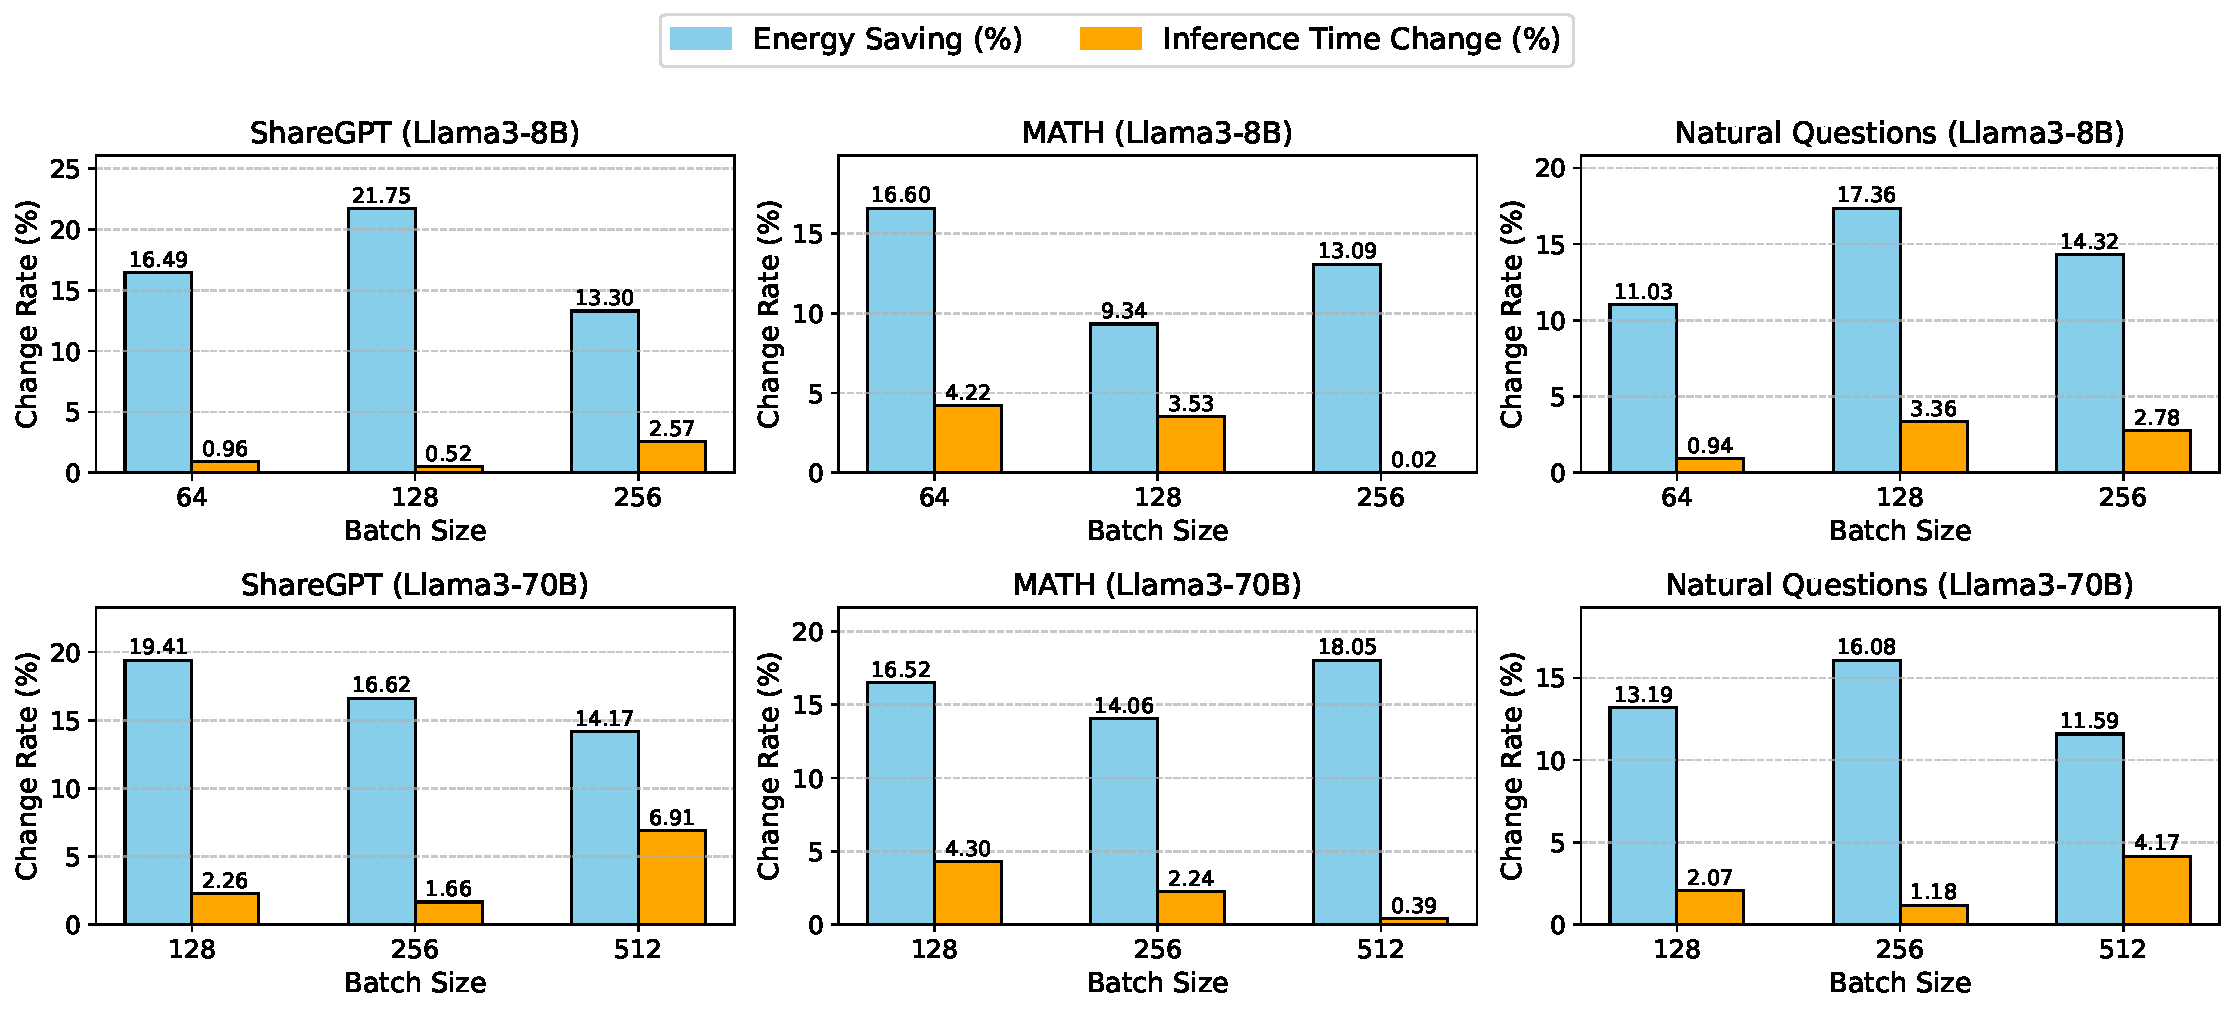
\includegraphics[width=1\linewidth]{figures/Energy_E2E_under_BatchSize_lyz_new_new_new_new_new.pdf}
    \caption{\bylyz{Energy efficiency and performance variations at different power levels across multiple datasets using Llama3-8B model, Llama3-70B and XXX. 
    Positive numbers indicate energy efficiency improvements and performance degradation.
    }\lyzcheck{3*3 Figures similar to this. But add XXX model in the last row. And change the label, with three labels, including energy efficiency, inference time and throughput. The x is Batch Size, and y is Change Ratio. Different row means different model, and different column means different DataSet. }}
    \label{latency_energy}
\end{figure*}



\subsection{Experimental Setup}

\textbf{Hardware.}
The experiments have been conducted on two workstations.
The first is equipped with an Intel Xeon Gold 6326 CPU running at 2.90 GHz and four NVIDIA RTX 3090 GPUs, each with 24 GB of memory.
The second is equipped with Intel Xeon Gold 6348 CPU running at 2.60 GHz and eight A100 GPUs, each with 40 GB of memory.
Both workstations are operating on Ubuntu 22 and have utilized the PyTorch 2.3.0 framework with CUDA 12.4 to leverage GPU acceleration.

% In the experiment, we select two mainstream open-source LLM models for evaluation: Llama3-8B and Llama3-70B.
% % \bylyz{The first two models are executed on the first workstation, while the last is on the second workstation.}
% Llama3-8B is executed on the RTX3090, while Llama3-70B is on A100.
% The workload is derived from three datasets: Natural Questions\cite{kwiatkowski2019natural}, ShareGPT\cite{chiang2023vicuna}, and MATH\cite{hendrycks2021measuring}. 
% The first two datasets are natural language question-answering benchmarks, while MATH focuses on mathematical reasoning. 
% These datasets are widely recognized in the field and are commonly used to evaluate LLM capabilities such as language understanding, reasoning and handling long-context scenarios.
% For every dataset, we randomly select input (i.e., the questions) from the dataset to simulate users' requests.

\bylyz{
\textbf{Model.} In the experiment, we select three mainstream open-source LLM models using BF16 precision for evaluation: Llama3-8B, Llama3-70B, and XX.
Specifically, Llama3-8B is deployed on RTX 3090 GPUs using vLLM, Llama3-70B is deployed on A100 GPUs using SGLang, and XX is deployed on RTX 3090 GPUs using SGLang.
The batch size is set to {64, 128, 256} for Llama3-8B, {128, 256, 512} for Llama3-70B, and {XXX, XXX, XXX} for XX, considering both memory capacity and inference efficiency.
We use CUDA events to record the execution time of each batch, and its average value is utilized as $T$ in the $TFPrediction Model$. 
}

\bylyz{
\textbf{Workload.}
The workload is derived from three datasets: Natural Questions\cite{kwiatkowski2019natural}, ShareGPT\cite{chiang2023vicuna}, and MATH\cite{hendrycks2021measuring}. 
The first two datasets are natural language question-answering benchmarks, while MATH focuses on mathematical reasoning. 
These datasets are widely recognized in the field and are commonly used to evaluate LLM capabilities such as language understanding, reasoning and handling long-context scenarios.
For each dataset, we randomly sample inputs (i.e., user queries) to simulate real-world request patterns.
Specifically, we use XX requests for online evaluation, with a subset of 512 requests randomly selected for offline data profiling.
}

\bylyz{
\textbf{Metrics and Baseline.}
We take the end-to-end inference time and throughput (measured in generated tokens per second, tokens/s) as the key metric to evaluate the performance, while utilizing end-to-end energy consumption to evaluate the energy efficiency. 
For the energy consumption, we sample the real-time power usage of GPUs using the \textit{nvidia-smi} API provided by the NVIDIA GPU Driver at the granularity of 10 ms.
The sampled data is shown as a curve in Figure~\ref{power-runtime}, and the end-to-end energy is computed through the definite integration of the power curve.
To ensure measurement reliability, each experimental configuration is executed XXX times, with the average metrics reported as the final results.
We employ the default automatic DVFS mechanism as our baseline and evaluate our metrics against it.
}

% We use the question-answer pairs from the datasets for online evaluation and randomly select a portion of pairs for offline data profiling.
% In our experiments, the batch size is set to 64/128/256 for Llama3-8B and 128/256/512 for Llama3-70B, considering both memory capacity and efficient inference.
% During the profiling, 512 questions are randomly selected from the dataset as the input to the LLM inference engine.
% The execution time of each batch is recorded, and its average value is used for $T$ in the \emph{TFPrediction Model}. 
% \bylyz{
% We uses the cuda event to record he execution time of each batch, and its average value is used for $T$ in the \emph{TFPrediction Model}. 
% }
% }

% It is worth noting that, due to the CPU–GPU asynchronous execution mechanism in the inference engine, accurately measuring the execution time of individual stages is challenging.
% To address this, we insert explicit synchronization statements (e.g., \texttt{torch.cuda.synchronize}) during offline profiling, which improves the precision of batch execution time measurements.
% For online inference, however, these synchronizations are removed in order to avoid unnecessary stalls and maximize performance.



\subsection{Evaluation}


\begin{figure*}[t]
    \centering
    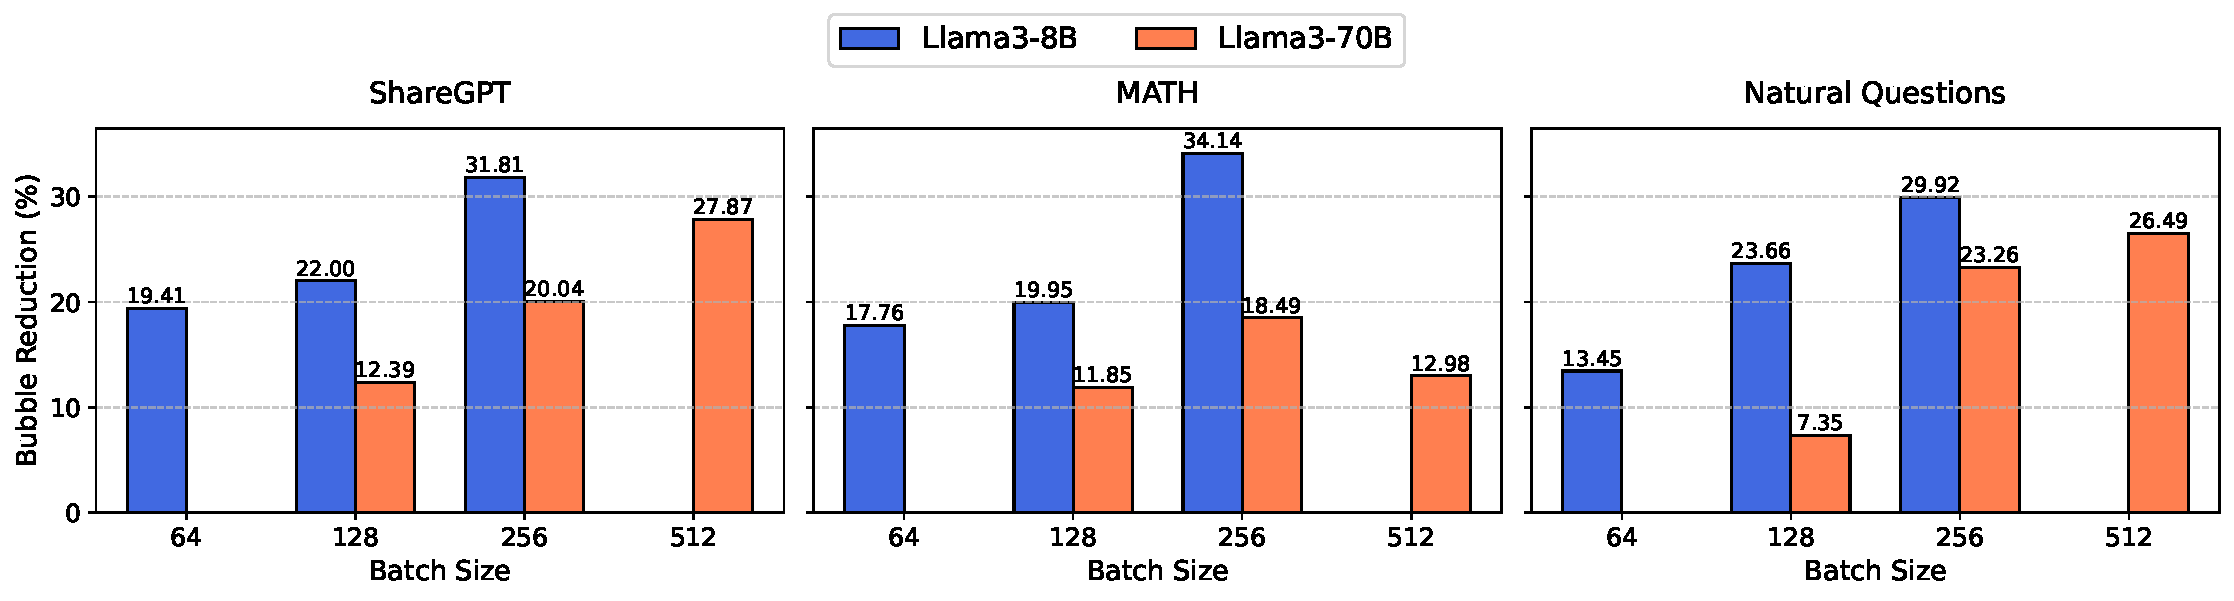
\includegraphics[width=\linewidth]{figures/IDLE_Computing_under_BatchSize_lyz_new_new_new_new.pdf}
    \caption{Percentage of bubble reduction across different batch size and datasets. \lyzcheck{(One figure is a model, x is batchsize, y is bubble reduction, different color means different dataset.)}}
    \label{IDLE_Computing}
\end{figure*}



% We take the end-to-end inference time and the energy consumption as the key metrics to evaluate the performance and the energy efficiency of the LLM inference system. 
% Specifically, the end-to-end inference time measures the time from the start of the first batch to the completion of all batches. 
% This also corresponds to the total execution time of the GPU that processes the last stage of the pipeline, i.e., GPU$_4$ as shown in Figure~\ref{timeline}.
% For the energy consumption, we sample the real-time power usage of GPUs using the \textit{nvidia-smi} API provided by the NVIDIA GPU Driver.
% The sampled data is shown as a curve in Figure~\ref{power-runtime}, and the total energy is computed through the definite integration of the power curve.
% \bylyz{
% We adopt the automatic DVFS mechanism as our baseline and compare these metrics against it.
% }



\subsubsection{Performance and Energy Efficiency}

\begin{table}
  \caption{\lyzcheck{The optimal frequency settings and \textit{TFPrediction Model} coefficient solved by \thisproj{}.}}
  \label{tab:fsettings}
  \begin{tabular}{ccccc}
    \toprule
    Model & 512 & 256 & 128 & 64 \\
    \midrule
    Llama3-8B & -- & 5.39\%  & 4.40\%  & 1.71\%  \\
    Llama3-70B & 6.75\% & 3.12\% & 1.75\% & --  \\
    \bottomrule
  \end{tabular}
\end{table}

In Figure~\ref{latency_energy}, it shows the impact of \thisproj{} on the performance and energy efficiency for Llama3-8B, Llama3-70B and XXX across different datasets compared with DVFS. 
For simplicity of comparison, we normalized the data against the baseline.
The above bars in the figure represent the energy efficiency improvement and performance degradation.
\lyzcheck{Table\ref{tab:fsettings} shows the corresponding optimal frequency solved by \thisproj{}}
The results demonstrate that \thisproj{} consistently achieves significant energy efficiency improvements across all three datasets, regardless of the batch size and the LLM model.

Notably, the energy efficiency improvements reach their highest at XXX\% with the batch size of XXX on the XXX dataset using the XXX model.
Across all three datasets and on average, XXX\% improvements can be achieved for the Llama3-8B, XXX\% for the Llama3-70B and XXX\% for the XXX.
This is also reflected by the minimal performance variation observed across different batch sizes.
Given that batch size is typically constrained by the GPU memory capacity in real-world scenarios, these results show that \thisproj{} can function well under varying memory limitations.

The XXX bars and XXX bars in the figure show the inference time and throughput variations respectively. 
Positive values indicate an decrease in the performance, whereas shorter bars signify better.
%These variations may result from model deviations, 
These variations may be caused by the imprecision of the analytical model, which can lead to an overestimation of pipeline bubbles and subsequent over-adjustment of the frequency.
%which can introduce performance overhead.
Nevertheless, the results show that the introduced fluctuation in the performance is quite minimal—approximately XX\% and XX\% on inference time and throughput on average—indicating that the analytical model is quite accurate and the impact of the energy efficiency improvement on the inference time is rather small.
% For those bars below zero, they are mostly caused by the performance variation and the measurement noises during the LLM inference.
Besides, inherent performance variations and the measurement noises can also cause the system’s performance to fluctuate to some extent.
% For those bars exhibiting slightly larger variations, they may also be caused by the performance variation and the measurement noises during the LLM inference.


% To further investigate the impact of power cap on the system, we select a specific inference engine configuration and enumerate different power cap.
To further investigate the impact of frequency adjustment on the system, we select a specific inference engine configuration and evaluate it under different frequency settings.
We vary the frequency from XXX to XXX in an increment of XXX for the Llama3-70B and XXX, using XXX dataset.
In each setting, inference time and energy consumption are measured.
The results are shown in Figure~\ref{power_lantency_math}.
As the frequency decreases (from XXX to XXX), a larger proportion of pipeline bubbles is mitigated, resulting in sustained energy efficiency improvement, while the overall system performance remains largely unaffected.
However, when the frequency falls below a critical threshold (from XXX to XXX), the execution time of the preceding stages surpasses that of the last stage, thereby becoming the system's bottleneck.
Consequently, system performance drops sharply, and the associated energy efficiency improvement diminish, potentially resulting in negative gains.

\bylyz{
Table shows our solved frequency settings using \thisproj{}.
It shows that ...(some analysis).
% It also shows that the optimal frequency setting lies between XXX and XXX, with the optimal value close to XXX.
% We use \thisproj{} to calculate the frequency that exactly matches the execution time of the preceding stage to the last stage.
% The predicted frequency is XXX, which closely aligns with the experimental results.
}

\subsubsection{Reduction of Bubbles}
\label{sec:evaluatebubble}

% \begin{figure*}[t]
%     \centering
%     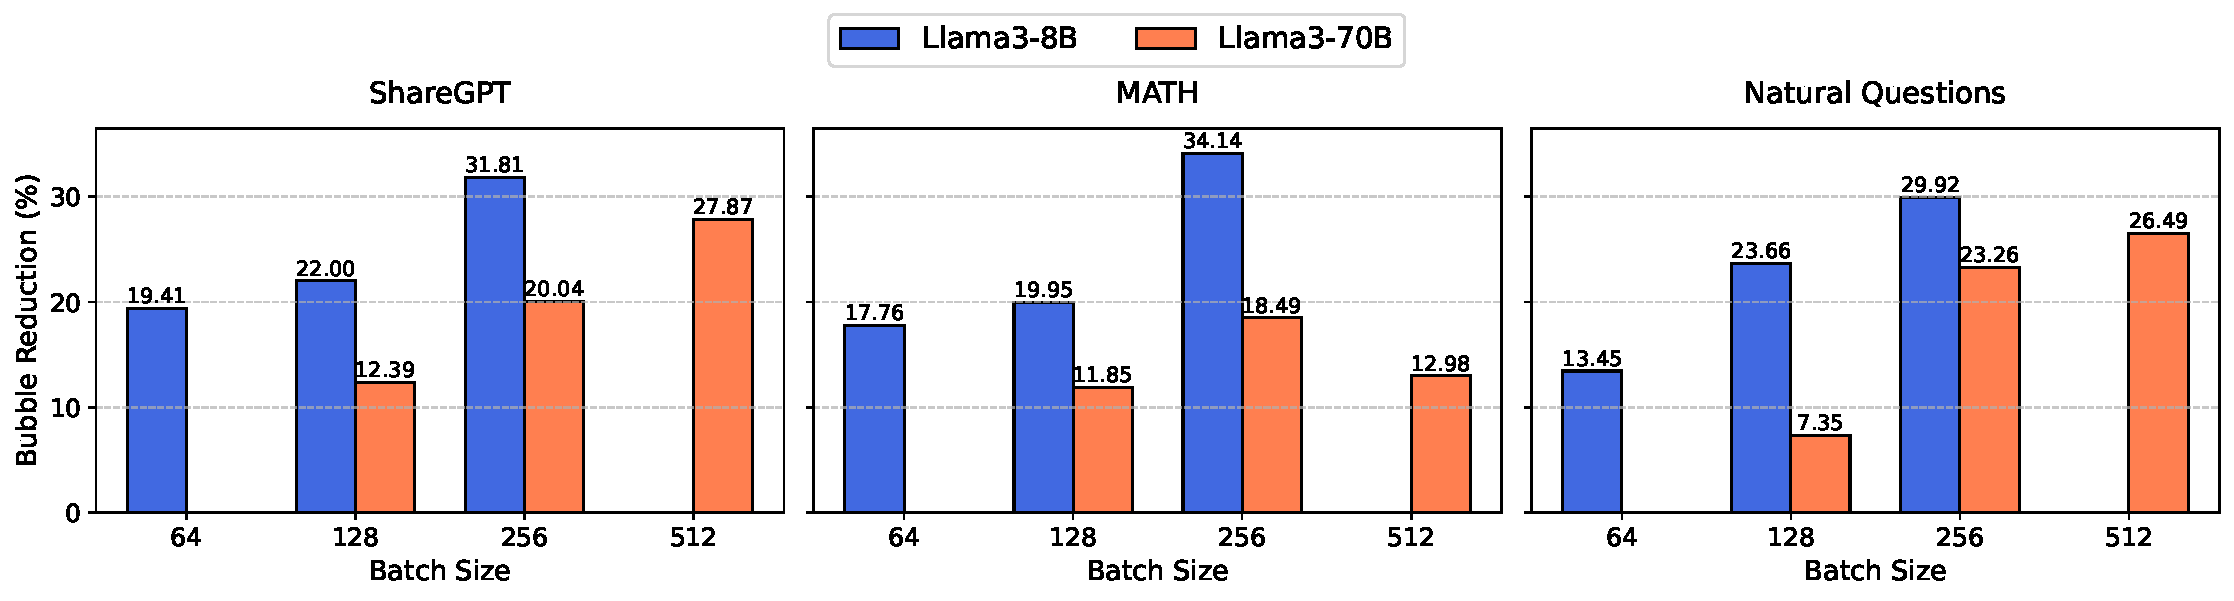
\includegraphics[width=\linewidth]{figures/IDLE_Computing_under_BatchSize_lyz_new_new_new_new.pdf}
%     \caption{Percentage of bubble reduction across different batch size and datasets.}
%     \label{IDLE_Computing}
% \end{figure*}

% Figure 13
% \begin{figure}[t]
%     \centering
%     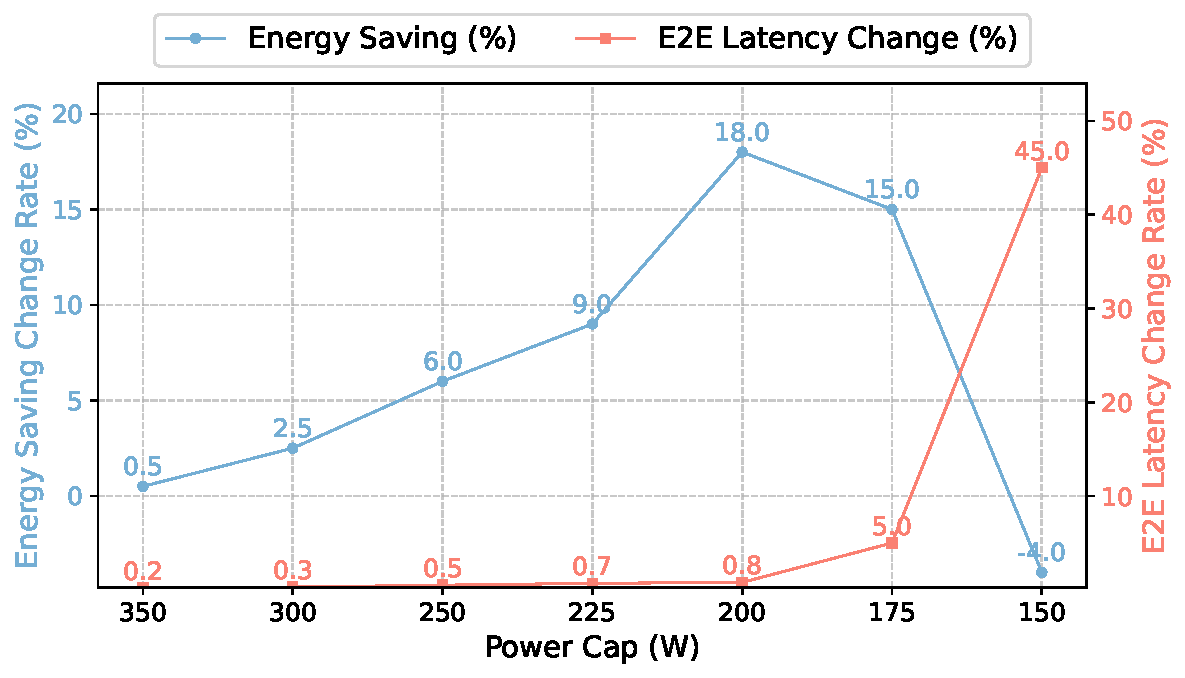
\includegraphics[width=0.9\linewidth]{figures/power_lantency_math_lyz_new_new_new.pdf}
%     \caption{Latency and energy reduction on the MATH dataset using Llama3-70B and a batch size of 512 with different power cap settings.}
%     \label{power_lantency_math}
% \end{figure}

% Figure 14
% \begin{figure}[t]
%     \centering
%     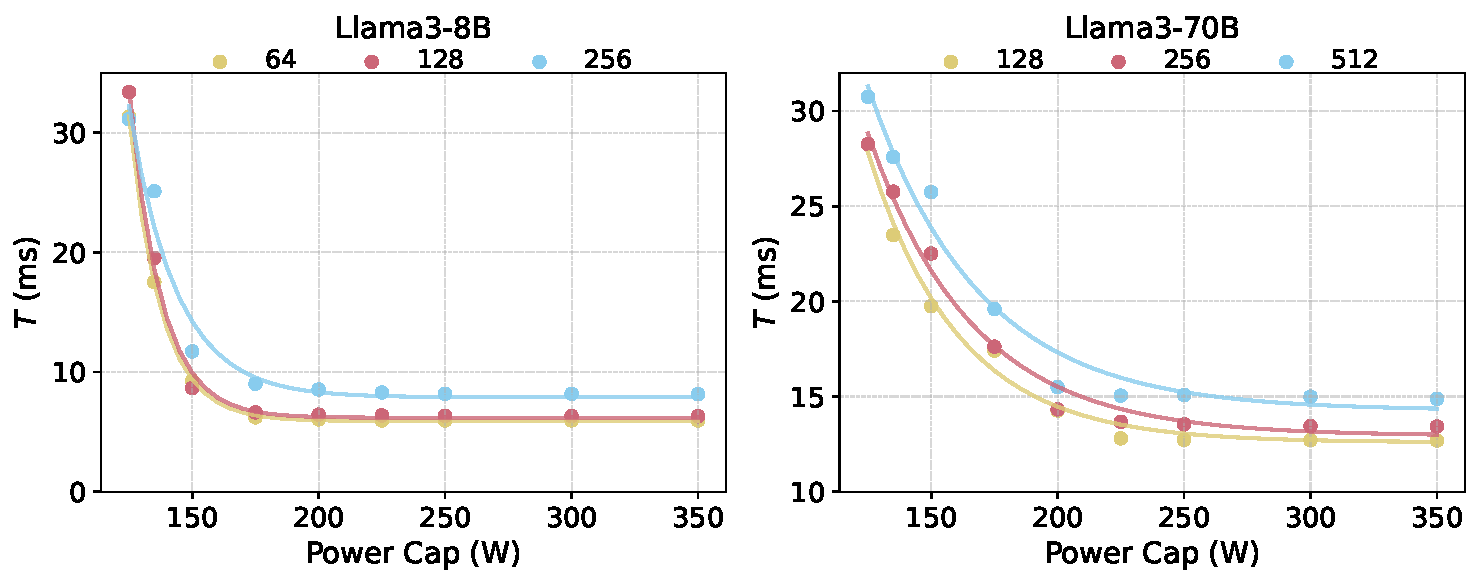
\includegraphics[width=\linewidth]{figures/execution_time_prediction_new_new.pdf}
%     \caption{Curve fitting for the relationship between power cap $P$ and batch stage execution time $T$ across different batch size, models, and platforms. The scatter points represent actual measured values, while the curves are derived from the fitted model.}
%     \label{fig:curvefit}
% \end{figure}


% Figure 13 and 14
\begin{figure}[t]
    \centering
    \begin{minipage}[t]{0.48\textwidth}
        \centering
        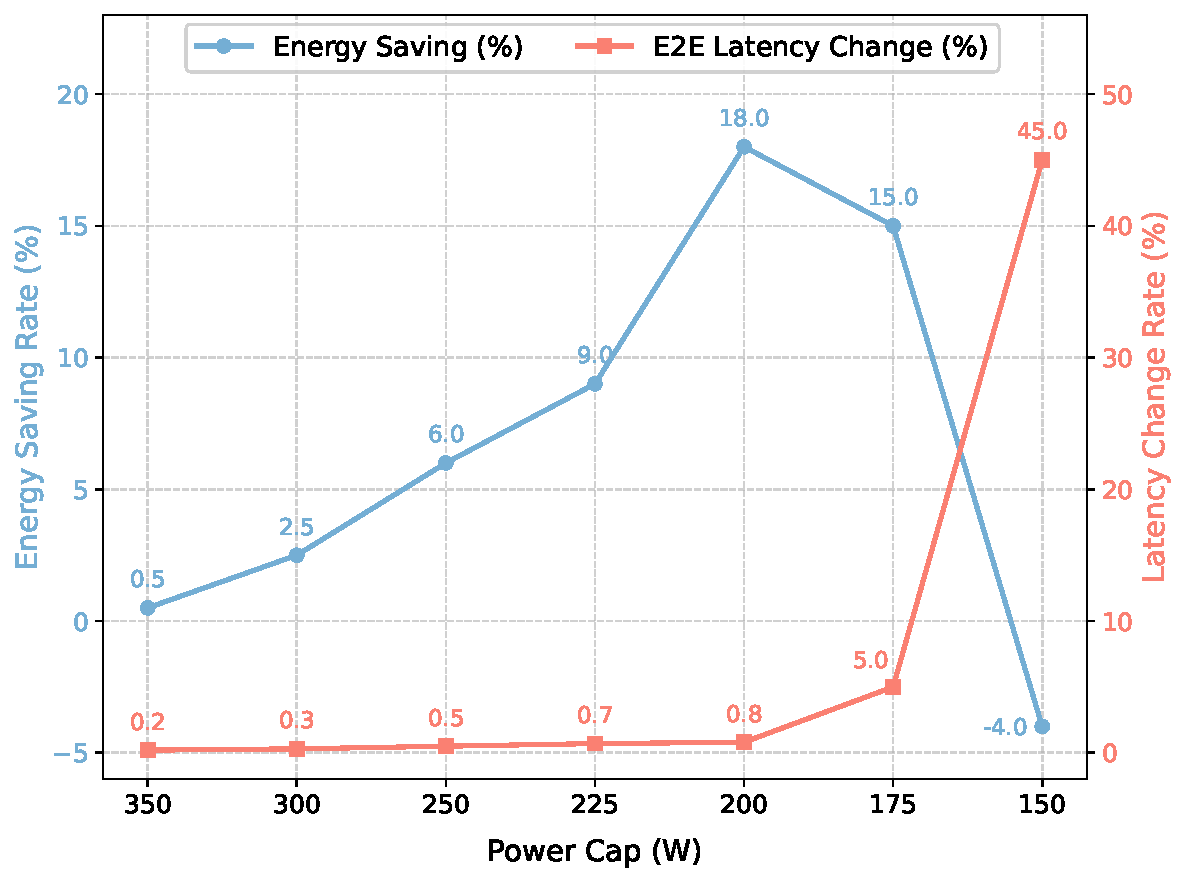
\includegraphics[width=\textwidth]{figures/power_lantency_math_lyz_new_new_new_new_new_new.pdf}
        \caption{\bylyz{Enegry efficiency and performance variations on the XXX dataset using Llama3-70B (batchsize: XX) and XXX (batchsize: XX) with different frequency settings.
        \lyzcheck{(Two figures. The top is about Llama3-70B, while the bottom is about XXX. The X is Frequency Settings and left y is Energy Efficiency and right y is Inference Time.(There use the actual value not percentage.))}}}
        \label{power_lantency_math}
    \end{minipage}
    \hspace{0.02\textwidth}
    \begin{minipage}[t]{0.48\textwidth}
        \centering
        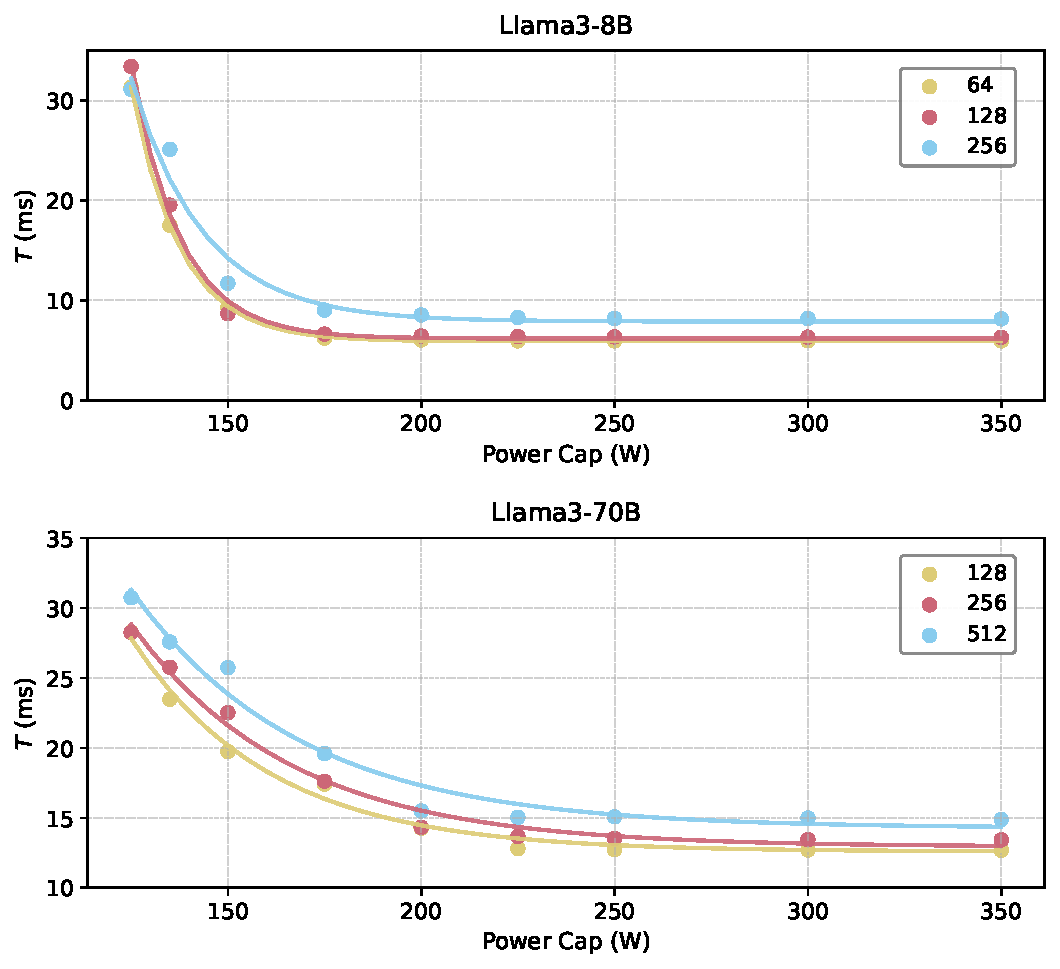
\includegraphics[width=0.87\textwidth]{figures/execution_time_prediction_new_new_new.pdf}
        \caption{Curve fitting for the relationship between frequency $f$ and stage execution time $T$ across different batch size, models, and platforms. The scatter points represent actual measured values, while the curves are derived from the fitted model.
        \lyzcheck{Three figures, left Llama3-8B, middle Llama3-80B, right XXX. The x is $f$, the y is $T$. Different Color Means different Batch Size.}
        }
        \label{fig:curvefit}
    \end{minipage}
\end{figure}

% Figure 13 and 14
% \begin{figure}[t]
%     \centering
%     % 使用 [b] 确保两个 Caption 的顶端是对齐的，视觉上更整齐
%     \begin{minipage}[b]{0.48\linewidth}
%         \centering
%         % 统一限制高度（如 3.8cm），keepaspectratio 防止变形
%         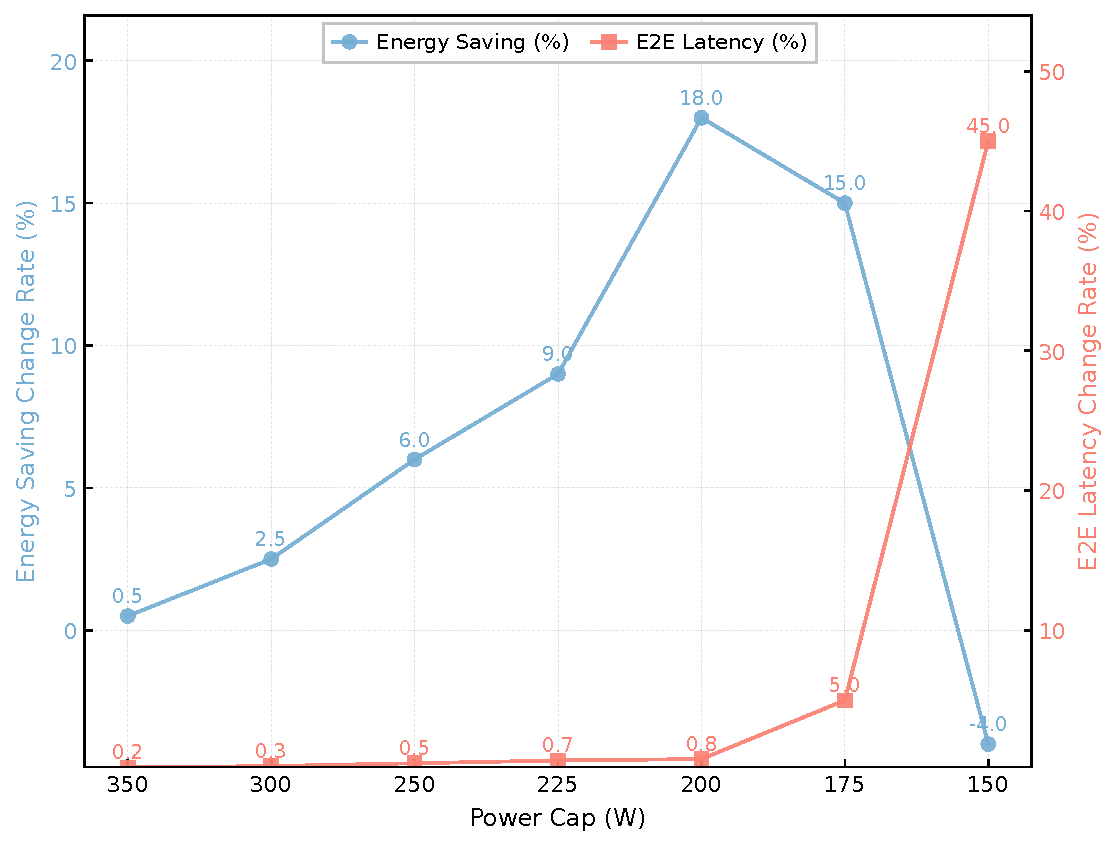
\includegraphics[width=\linewidth, height=3.8cm, keepaspectratio]{figures/power_lantency_math_lyz_new_new_new_new.pdf}
%         \vspace{-6pt} % 缩小图片与标题之间的空隙
%         \caption{\small Latency and energy reduction on the MATH dataset.} % 建议精简标题，详细描述放正文
%         \label{power_lantency_math}
%     \end{minipage}
%     \hfill % 自动撑开左右间距
%     \begin{minipage}[b]{0.48\linewidth}
%         \centering
%         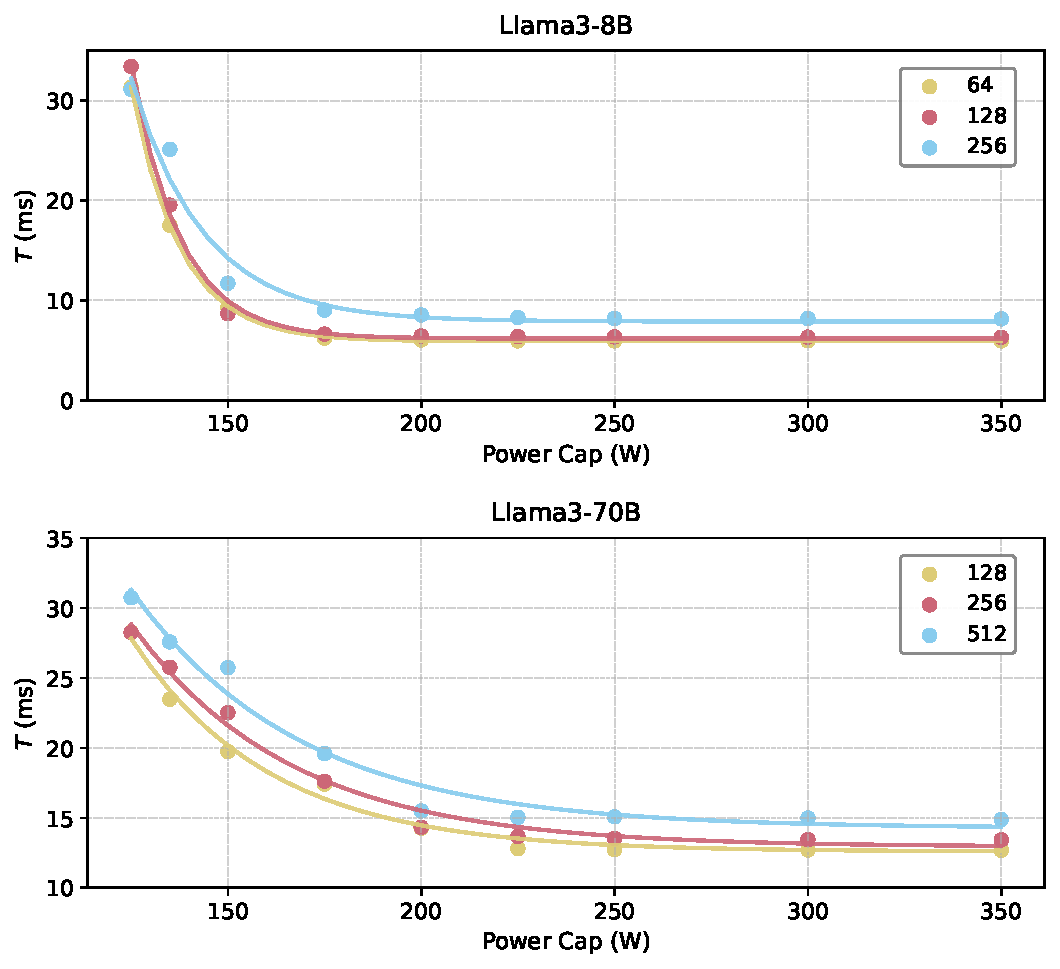
\includegraphics[width=\linewidth, height=3.8cm, keepaspectratio]{figures/execution_time_prediction_new_new_new.pdf}
%         \vspace{-6pt}
%         \caption{\small Curve fitting for power cap $P$ and stage time $T$.}
%         \label{fig:curvefit}
%     \end{minipage}
% \end{figure}

To further understand the energy efficiency improvement, we evaluate the proportion of pipeline bubbles before and after the adjustment of the frequency settings using \thisproj{} to verify its impact on the pipeline performance. 
Figure~\ref{IDLE_Computing} shows the percentage of reduction across multiple datasets and batch size.
In the experiment, we record the start and the end time of every batch in each stage. 
In each stage, the duration between the end time of a batch and the start time of the following batch is identified as a pipeline bubble.
While the duration between the start time of the first batch in the first stage and the end time of the last batch in the final stage is recorded as the total execution time for the inference.
Finally, the percentage of the time consumed by pipeline bubbles is calculated.
The figure illustrates the reduction in the pipeline bubbles under various conditions. 

The most significant reduction occurs with a batch size of XXX and XXX dataset on XXX that reaches XXX\%. 
On average, a XXX\% reduction in bubbles can be achieved across three datasets and various batch sizes using the Llama3-8B model, XXX\% on Llama3-70B and XXX\% on XXX.
This demonstrates that lowering frequency can effectively extend the computation time to squeeze out bubbles and reduce their proportion in the pipeline without affecting the total inference time.

It is important to note that GPU idle time is not solely caused by pipeline bubbles. 
Factors such as communication delays, abnormal requests with extremely long contexts, and the asynchronous execution mechanism also contribute to GPU idling. 
Consequently, it is not possible to completely eliminate GPU idle time using \thisproj{}.


\subsubsection{Model Accuracy and Universality}
\label{sec:evaluatecurvefitting}


We also evaluate the accuracy of the \textit{TFPrediction Model} to validate its ability to correlate the performance and its energy efficiency across various configurations including different batch size. 
%The evaluation involves comparing the model's prediction with the actual data to ensure that it accurately represents the system's behavior under different conditions.
%
Note that, as discussed in Section 3.2, we purposely exclude the batch size as a parameter used in the \emph{TFPrediction Model} because of its discrete nature.

The results are illustrated in Figure~\ref{fig:curvefit}. 
In the figure, each point of different colors represents the average execution time, denoted as $T$ in the \emph{TFPrediction Model}, for a specific batch size and frequency setting.
The curve of the same color represents the values predicted using the \textit{TFPrediction Model}.
%results generated through the curve-fitting process.
%The figure demonstrates 
It shows a high degree of agreement between the predicted value and the measure data point, validating the effectiveness of the curve-fitting method used in \thisproj{}.

To further validate the accuracy and the universality of \thisproj{}, a dataset is constructed for each batch size on an LLM by combining the measured results from all three datasets.
In each measurement, the frequency $f$ and the average batch execution time $T$ are recorded.
For each batch size and model, we make 11 measurements and collect 11 pairs of $f$ and $T$ for each dataset.
In a dataset, 60\% of the data is randomly selected for the curve fitting, while the remaining data is used to evaluate the resulted curve. 
We then calculate their \emph{Mean Absolute Percentage Error (MAPE)}.

\begin{table}
  \caption{Mean absolute percentage errors (MAPEs) of different batch size and LLM models using the ShareGPT dataset (lower is better).}
  \label{tab:mape}
  \begin{tabular}{ccccc}
    \toprule
    Model & 512 & 256 & 128 & 64 \\
    \midrule
    Llama3-8B & -- & 5.39\%  & 4.40\%  & 1.71\%  \\
    Llama3-70B & 6.75\% & 3.12\% & 1.75\% & --  \\
    \bottomrule
  \end{tabular}
\end{table}


% \bygxl{
The results are shown in Table~\ref{tab:mape}. 
% For the evaluated models of Llama3-8B and Llama3-70B, it achieves an MAPE as small as 6.75\% across all batch sizes. 
For the evaluated models, including Llama3-8B, Llama3-70B and XXX, it achieves an MAPE as small as 3.85\% on average. 
This demonstrates the stability of the correlation between $f$ and $T$, indicating that only 6 samples are sufficient to construct the model. 
Such lightweight profiling simplifies the deployment of the \thisproj{} framework.
Together with the high accuracy in predicting and setting the power caps, they make the \thisproj{} framework very practical and effective for pipelined-based LLM models running on most existing system configurations to achieve a good balance between the high performance and energy efficiency.
